\documentclass[12pt]{beamer}
\usepackage{amsmath, amsfonts, amssymb, amsthm}
\usepackage{graphicx}
\usepackage[brazilian]{babel}
\usepackage[utf8]{inputenc}
\usepackage{verbatim}
\usepackage{hyperref}
\usetheme{Madrid}

\title{Mini-Curso de \LaTeX\ \\ Aula 03 - Mais Formatação, Tabelas e Imagens}
\author{Fábio Meneghetti \and Pedro Caetano}
\date{4 de abril de 2016}

\begin{document}
\begin{frame}
  \titlepage
\end{frame}

\begin{frame}{Licença}
  Esta apresentação está licenciada com uma Licença Creative Commons Atribuição-CompartilhaIgual 4.0 Internacional.
  \begin{center}
    
\includegraphics[scale=0.3]{../license.png}
  \end{center}
\end{frame}

\begin{frame}[fragile]{Resposta do Exercício}

  \begin{verbatim}
    \usepackage[top=3px,
                left=2cm,
                right=1em,
                bottom=2pt]{geometry}
  \end{verbatim}

\end{frame}

\begin{frame}
  \tableofcontents
\end{frame}

\begin{frame}[fragile]{Alinhamento do texto}
  \section{Formatação (continuação)}
  O alinhamento pode ser feito usando um ambiente ou um comando. O comando faz que todo o texto o texto a partir daquele ponto seja alinhado, e é recomendado que se use apenas dentro de algum outro ambiente, ou dentro de \{ e \} (como veremos em tabelas e figuras). Para um texto normal, o ambiente é mais recomendado.
  \begin{center}
    \begin{tabular}{ccc}
    \textbf{Alinhamento} & \textbf{Ambiente} & \textbf{Comando}\\
    À esquerda & flushleft & \verb+\raggedright+\\
    À direita & flushright & \verb+\raggedleft+\\
    Centralizado & center & \verb+\centering+\\
    \end{tabular}
  \end{center}
\end{frame}

\begin{frame}[fragile]{Comandos para o texto}
  \begin{itemize}
    \item \textit{itálico}: \verb+\textit{texto}+
    \item \textbf{negrito}: \verb+\textbf{texto}+
    \item \underline{sublinhado}: \verb+\underline{texto}+
    \item \textsc{Letra de forma}: \verb+\textsc{texto}+
    \\[.5cm]
    O comando para tamanho da fonte muda o tamanho de tudo dentro do ambiente, ou dentro de \{ e \}. Portanto para deixar apenas um texto em tamanho grande, é preciso usar \verb+{\Large texto}+
    \item Comandos em ordem crescente: tiny, scriptsize, footnotesize, small, normalsize, large, Large, LARGE, huge, Huge
  \end{itemize}
\end{frame}

\begin{frame}[fragile]{Espaçamento}

\begin{itemize}
  \item \verb+\\+ - quebra para a próxima linha. Tem uma opção para um espaço extra com \verb+\\[2cm]+
  \item \verb+\pagebreak+ - quebra de página
  \item \verb+\bigskip+, \verb+\medskip+ e \verb+\smallskip+ pulam certos espaço
  \item Vamos testar todas essas coisas no Exemplo 1!
\end{itemize}

\end{frame}

\begin{frame}[fragile]{Tabelas}
  \section{Tabelas}
  Para se iniciar uma tabela no \LaTeX, utiliza-se um ambiente chamado tabular. A parte do \verb+\begin+ tem duas entradas, uma é nome do ambiente (tabular) e a outra é o alinhamento de cada coluna (l, c ou r), separados por um espaço:
  \begin{verbatim}
  \begin{tabular}{l c c}

  \end{tabular}
  \end{verbatim}
\end{frame}

\begin{frame}[fragile]
  Cada linha do texto nesse ambiente será uma linha da tabela, e o fim da linha deve ser indicado com um \verb+\\+.

  Os elementos na linha devem ser separados pelo símbolo \verb+&+:
  \begin{verbatim}
  \begin{tabular}{l c}
    Corrente [A] & Tensão [V]\\
    15 & 30\\
    10 & 20\\
  \end{tabular}
  \end{verbatim}

  (Ver resultado no Exemplo 2)
\end{frame}

\begin{frame}[fragile]
  Para adicionar linhas verticais, basta utilizar o símbolo \verb+|+ entre as letras da segunda entrada do ambiente tabular.

  \textbf{Ex:} \verb+\begin{tabular}{|l|c|c|}+

  \medskip

  Para adicionar linhas horizontais, basta adicionar \verb+\hline+ entre os valores da tabela.

  \textbf{Ex:}
  \begin{verbatim}
  \begin{tabular}{|l|c|}
    \hline
    Corrente & Tensão\\
    \hline
    15 & 30\\
    \hline
  \end{tabular}
  \end{verbatim}
  (Tente no Exemplo 2!)
\end{frame}

\begin{frame}[fragile]
  Para adicionar legendas, labels, e para se definir uma posição da tabela, é recomendável colocar o ambiente tabular dentro de um ambiente table:
  \begin{verbatim}
  \begin{table}[opções]
    \begin{tabular}{...}
      ...
    \end{tabular}
  \end{table}
  \end{verbatim}
\end{frame}

\begin{frame}[fragile]
  \begin{itemize}
    \item As opções indicam o posicionamento da tabela, e são dadas por:
    \begin{itemize}
      \item \textbf{h} - Onde o código se encontra
      \item \textbf{t} - No topo da página
      \item \textbf{b} - No fim da página
      \item \textbf{!} - Tira algumas restrições do tipo tabela (tente usar se algo não está saíndo do jeito que você quer)
    \end{itemize}
    \item É possível colocar um comando de alinhamento, como \verb+\centering+ antes de começar o ambiente tabular
    \item Ainda é possível adicionar um \verb+\caption{texto}+ para colocar uma legenda na tabela
    \item Para fazer referência a essa tabela (como explicado na Aula 2), use \verb+\label{table:nome_do_marcador}+
  \end{itemize}
\end{frame}

\begin{frame}[fragile]
  \textbf{Exemplo:}
  \begin{verbatim}
  \begin{table}[!h]
    \centering
    \begin{tabular}{...}
      ...
    \end{tabular}
    \caption{Esta á uma tabela muito elegante}
    \label{table:elegancia}
  \end{table}
  \end{verbatim}

  \textbf{Dica:} Extensão do OpenOffice Calc2LaTeX
\end{frame}

\begin{frame}[fragile]{Listas}
  \section{Listas}
  \begin{itemize}
    \item Existem dois ambientes para listas, o itemize e o enumerate. A diferença entre os dois é que o enumerate é numerado e o itemize não.
    \item Dentro do ambiente, coloque o comando \verb+\item+ no começo de cada linha que você quer que seja um item
    \item Ver Exemplo 3!
  \end{itemize}
\end{frame}

\begin{frame}[fragile]{Figuras}
  \section{Figuras}
  Introduzimos figuras em documentos \LaTeX\ usando o comando \verb+\includegraphics+, do pacote graphicx, cuja sintaxe é
  \begin{verbatim}
    \includegraphics[parametro1=valor1, ...]
                               {arquivo_de_imagem}
  \end{verbatim}

  A entrada do comando deve possuir o caminho do arquivo de imagem a ser inserido relativo à pasta onde o arquivo tex se encontra. São suportados os formatos jpg, png, pdf e eps.

\end{frame}

\begin{frame}[fragile]
  Há várias opções disponíveis para o comando \verb+\includegraphics+. Algumas das mais usadas se encontram na tabela abaixo.
  \begin{center}
    \begin{tabular}{cc}
      \textbf{Opção} & \textbf{Efeito} \\
      width=x & Ajusta a largura da figura para x\\
      height=x & Ajusta a altura da figura para x\\
      scale=x & Ajusta a escala da figura para x\\
      angle=x & Gira a imagem x graus no sentido
      antihorário
    \end{tabular}
  \end{center}

  \textbf{Dica: } Às vezes é útil especificar a largura da imagem em função da largura do texto, que é obtida pelo comando \verb+\textwidth+. Assim, por exemplo, podemos fazer com que a largura da figura seja $80 \%$ da largura do texto com a opção \verb+width=0.8\textwidth+.
\end{frame}

\begin{frame}[fragile]

  \textbf{Exercício: } Inclua a imagem \emph{duck.jpg} no Exemplo 3 de forma a obter um resultado semelhante ao PDF do Exemplo 3.1\\
  \bigskip
  \pause
  \textbf{Solução: }
  \begin{verbatim}
    \begin{center}
      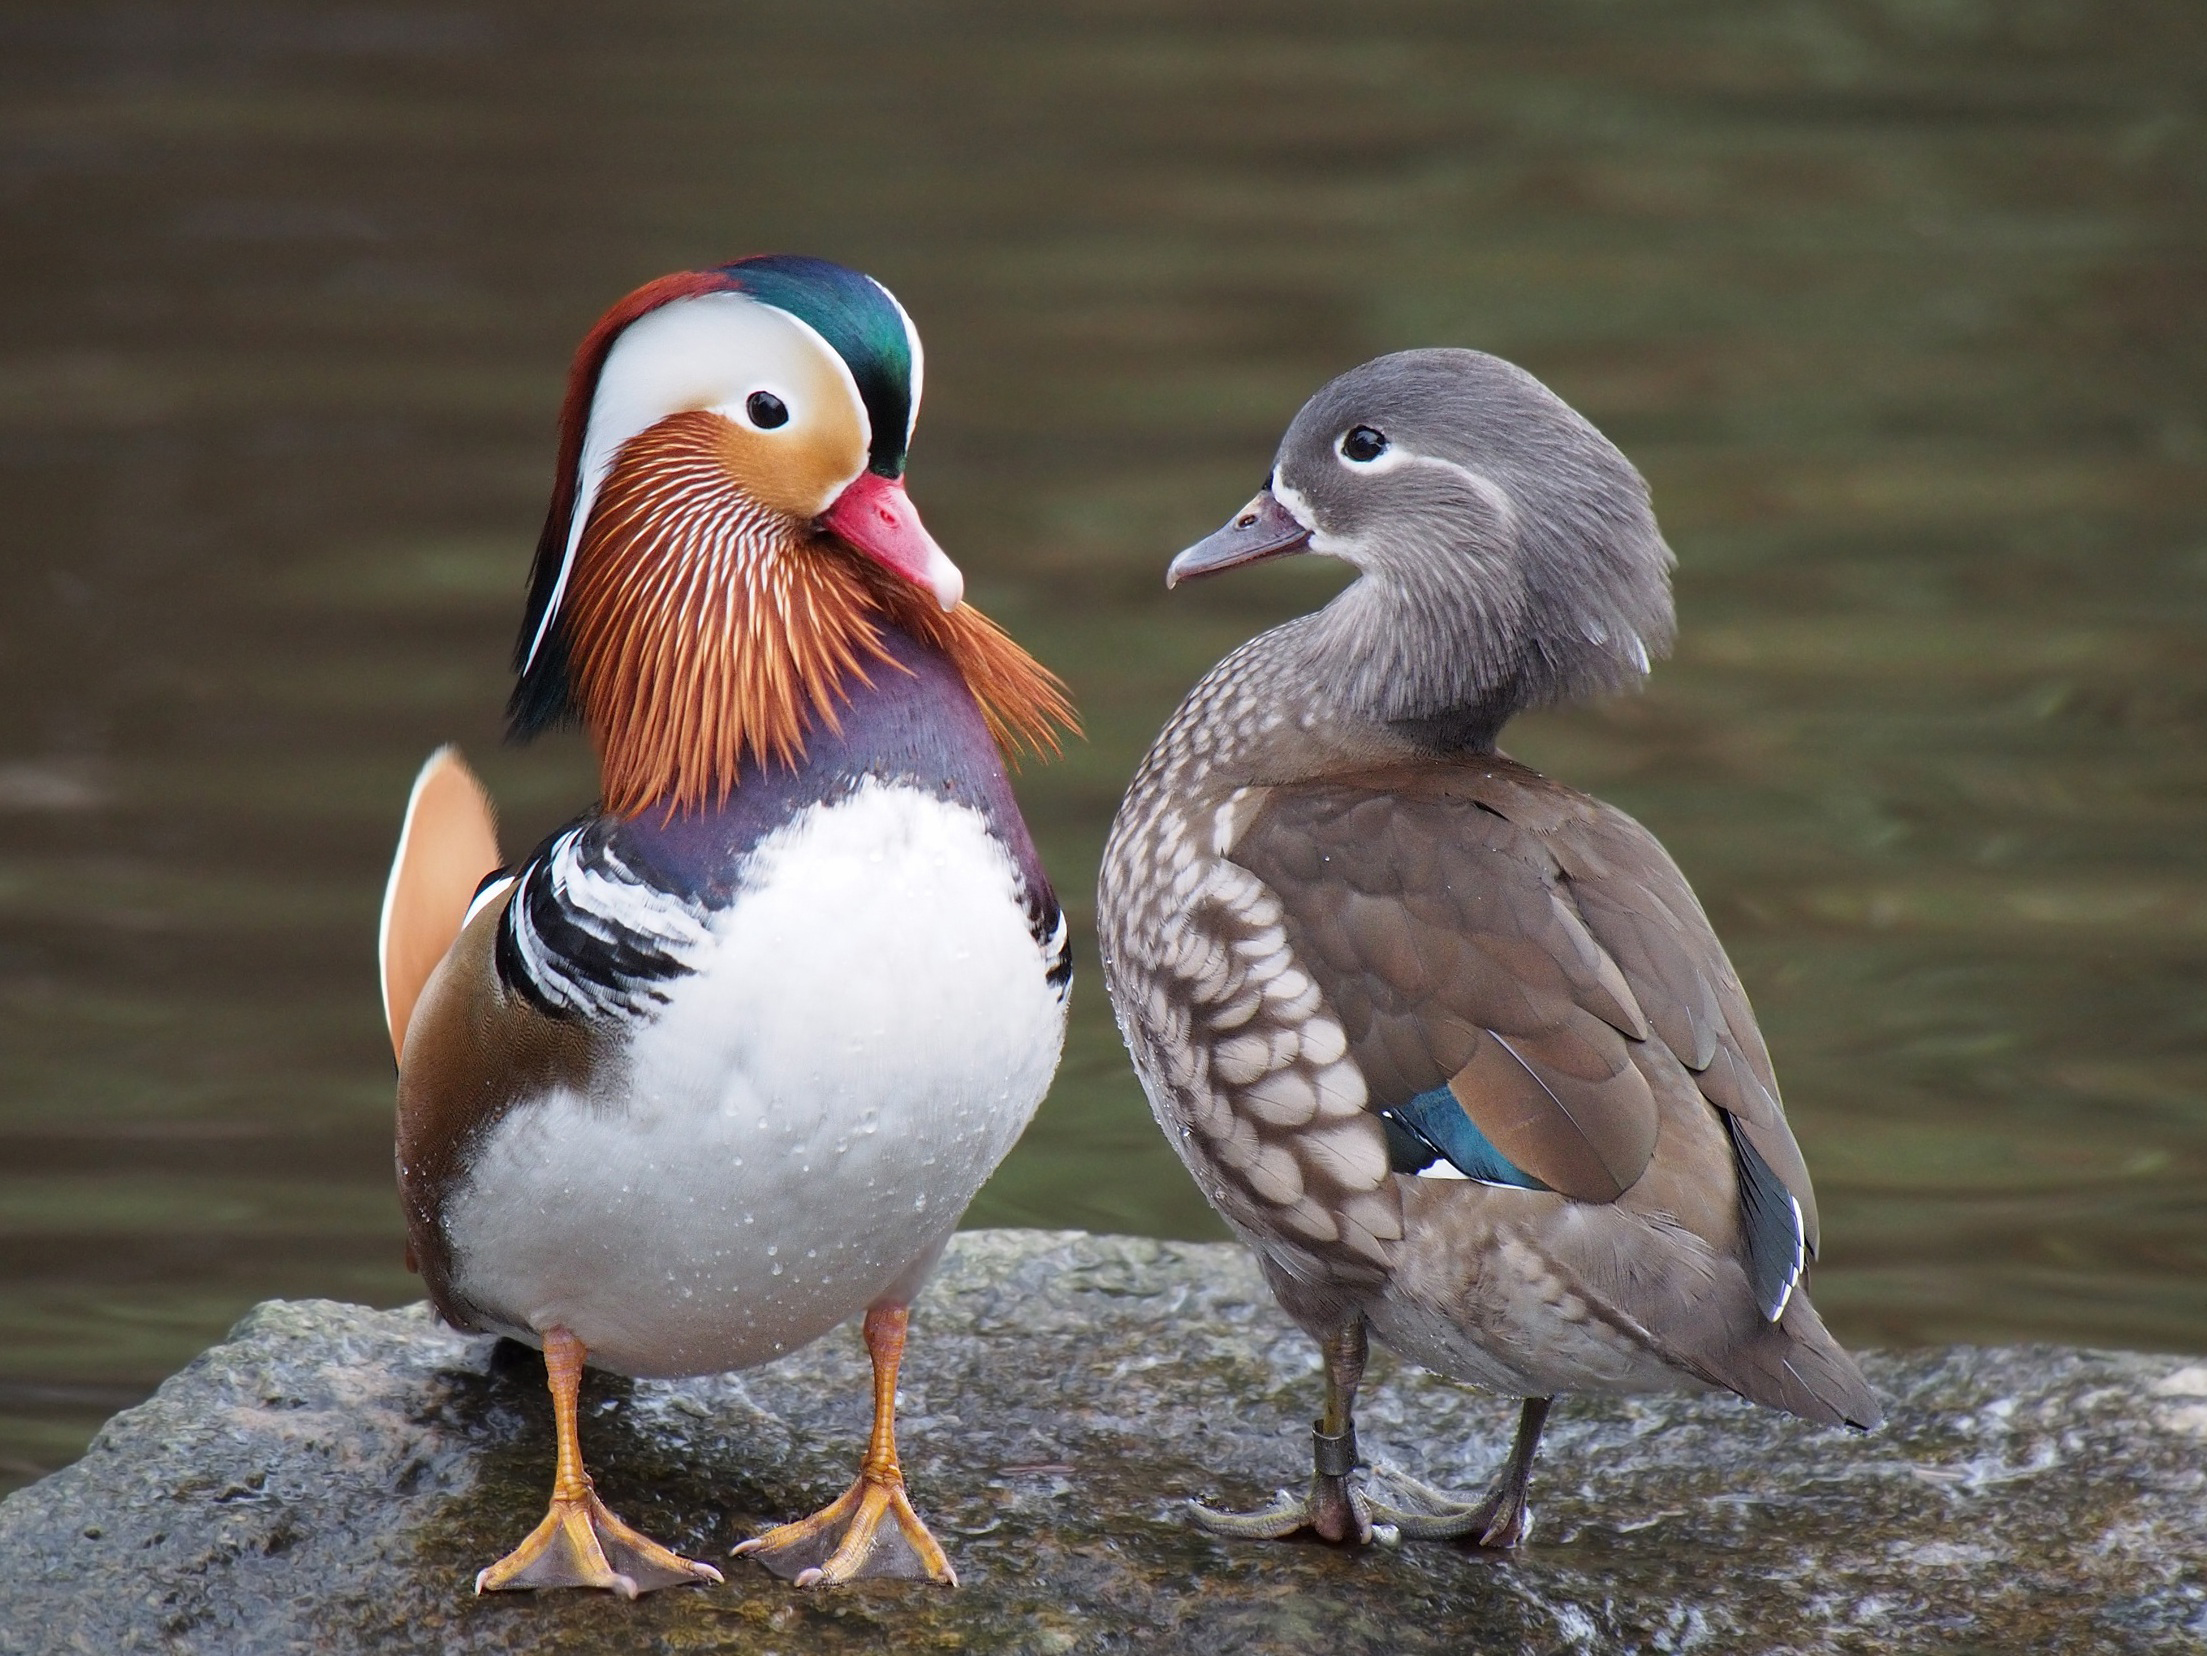
\includegraphics[width=0.65\textwidth]{duck}
    \end{center}
    Felicidade e elegância. Foto de Francis C. Franklin,
    licenciada sobre Creative Commons Atribuição-
    CompartilhaIgual 3.0 Não Adaptada. \\
  \end{verbatim}

\end{frame}

\begin{frame}[fragile]{Ambiente figure}
O ambiente figure desempenha para imagens papel semelhante ao do ambiente table para tabelas, permitindo que o \LaTeX\ ajuste a posição da imagem no texto e que possamos introduzir legendas e labels em nossas imagens.\\

\textbf{Sintaxe: }
\begin{verbatim}
\begin{figure}[htb]
  \centering
  \includegraphics[width=0.8\textwidth]{grafico}
  \caption{Legenda do gráfico.}
  \label{fig:grafico}
\end{figure}
\end{verbatim}

As opções do ambiente figure funcionam exatamente como as do ambiente table.
\end{frame}

\begin{frame}[fragile]
\textbf{Exercício: } Introduza o gráfico
 \emph{grafico\_patos.pdf} no Exemplo 2 usando o ambiente figure. Referencie o gráfico no texto usando labels.

\pause

\textbf{Solução: }
\begin{verbatim}
(cf. também a Figura \ref{fig:graf_pato}).

  \begin{figure}[htb]
    \centering
    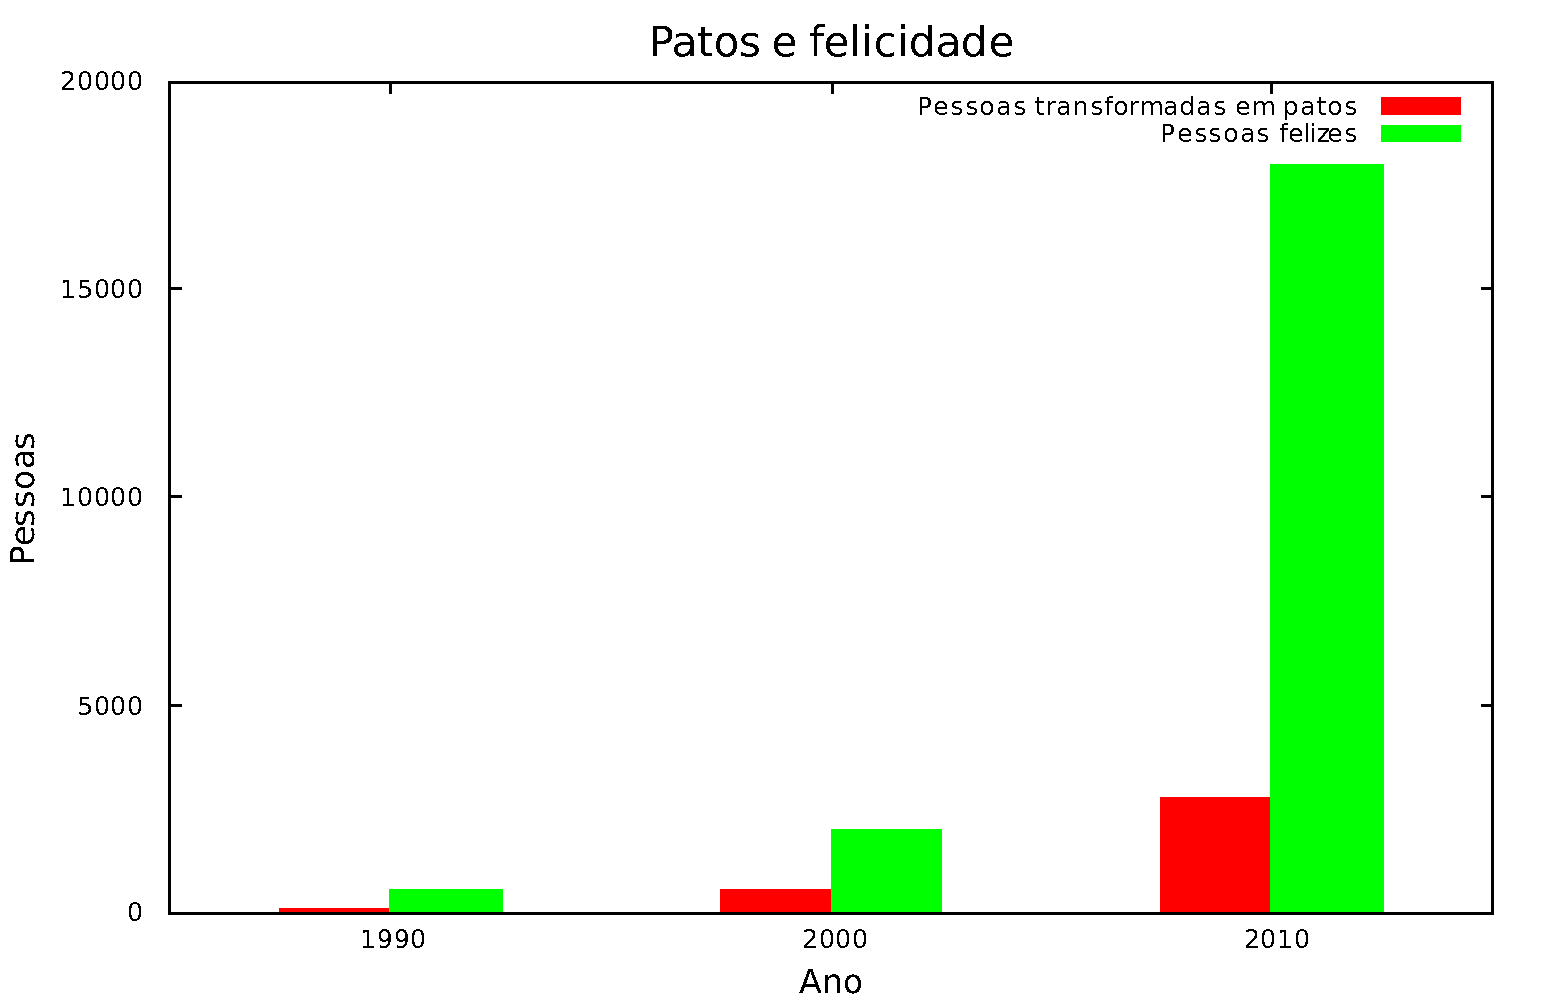
\includegraphics[width=\textwidth]{grafico_patos.pdf}
    \caption{Evolução recente do número de pessoas
    patonificadas e felicidade. Dados do último
    censo IBGE.}
    \label{fig:graf_pato}
  \end{figure}
\end{verbatim}

\end{frame}

\begin{frame}
  \begin{center}
    \large Obrigado!\\
    :)
  \end{center}
\end{frame}

\end{document}
